\documentclass[aspectratio=169]{beamer}

%
% Choose how your presentation looks.
%
% For more themes, color themes and font themes, see:
% http://deic.uab.es/~iblanes/beamer_gallery/index_by_theme.html
%
\mode<presentation>
\mode<presentation>
{
  \usetheme{Ilmenau}      % or try Darmstadt, Madrid, Warsaw, ...
  \usecolortheme{beaver} % or try albatross, beaver, crane, ...
  \usefonttheme{default}  % or try serif, structurebold, ...
  \setbeamertemplate{navigation symbols}{}
  \setbeamertemplate{caption}[numbered]
} 
\usepackage[english]{babel}
\usepackage[utf8x]{inputenc}
\usepackage{graphicx}
\usepackage{setspace}
\usepackage{tikz} \usetikzlibrary{snakes}
\usepackage{epstopdf}
\usepackage[round]{natbib}
\setbeamertemplate{enumerate items}[circle]
\setbeamertemplate{itemize items}[circle]
\setbeamertemplate{blocks}[rounded][shadow=false] 

\usepackage[english]{babel}
\usepackage[utf8x]{inputenc}
\title[Power and responsibility]{Falling house prices hurt incumbents}
\author{Frederik G. Hjorth \and Martin Vinæs Larsen}
\institute[UCPH]{\large{Department of Political Science \\ University of Copenhagen}}
\date[May 2015]{CVAP seminar, May 2015}

\begin{document}
	
	\begin{frame}
		\titlepage
	\end{frame}
	
	
\section{Politicized homes?}

	\begin{frame}
	%{Politicized homes}
	Key economic feature of post-industrial societies: mass home ownership.
	
	\vspace{0.2in} 

	\begin{itemize}
		\item main form of capital ordinary people have.
		\item key part of one's control over one's immediate context.
		\item often the focus of political rhetoric.
	\end{itemize}
	
		\vspace{0.2in} \pause
		
	$\rightsquigarrow$ but: relatively little research on how home ownership shapes political behavior.
		\end{frame}	
	
		\begin{frame}
		%{Politicized homes}
		\citet{ansell2014political}: house price appreciation reduces preferences for social insurance (see also \citealt{di2007formation,lewis2013compleat})	
						
		\vspace{0.2in}	\pause
						
		Here: house prices and \textit{incumbent government support}						
		
		\vspace{0.2in} \pause	
			
		``personal grievance hypothesis'': citizens blame (or credit) governments for personal grievances (favor) they experience; specifically, whether local house prices (appreciate) depreciate.
		
					\vspace{0.2in}	
					
				
			\end{frame}	
	\begin{frame}
	%{House prices as a personal economic grievance}
		
	
		
	At odds with received wisdom on economic voting: 
	\begin{block}{}
	``The political consequences of economic conditions are not carried by personally experienced hardships. Rather, a citizen's political response to economic conditions is mediated by judgments that are collectively oriented.'' \cite[p. 499]{kinder1979economic}	
	\end{block}

	
	\vspace{0.2in} \pause
	
	However, personal economic hardships previously studied have been
	\begin{enumerate}
	\item self-reported, and/or
	\item short-ranging (e.g. unemployment, reductions in income)
\end{enumerate}	

	\vspace{0.2in}
	
%	Conversely, if the value of your house changes this has profound and long lasting consequences; eviction, insolvency and ``credit-crunch''.	
			
	\end{frame}	
	
\section{Empirical setting}	
\begin{frame}
%{\insertsection}
In international comparison, DK's housing bubble exceptionally volatile:
\begin{center}
\includegraphics<1>[width=0.8\textwidth]{../../figures/intcomparison.png}
\end{center}
\end{frame}	
	
	
\section{Data}	
\begin{frame}
%{Data on house prices I}
House prices are hard to measure
\begin{itemize}
\item for individual home, unobserved outside of purchase/sale \pause
\item plausible proxy: realized house prices in local context \pause

$\rightsquigarrow$ context effect \emph{and} personal experience
\end{itemize}
% - no one knows exactly what a house costs until it is on the market - but good proxy is how much houses in the same area costs. 

\vspace{0.2in} \pause

Data on municipal selling prices from the Danish Mortgage Banks' Federation covering twenty years (1992:2013). 
%Covers important housing-bubble. 

%\vspace{0.2in}
%The data is on the municipal level and covers the average selling price of houses and condos in the municipality in a given quarter (mean number of sales per quarter is 112).

%\vspace{0.2in}
%This gives us a good indicator of what we want to know; namely, whether home-owners should expect the value of their house (or condo) to have appreciated or depreciated. 

\end{frame}	

\begin{frame}
%{Data on house prices II}
\begin{center}
\includegraphics<1>[width=0.9\textwidth]{../../figures/priceacrossmuni.eps}
\includegraphics<2>[width=0.9\textwidth]{../../figures/manylines_oneplot.eps}	
\includegraphics<3>[width=0.9\textwidth]{../../figures/prices_histogram.eps}	
\pause[3]

$\mu=0.05$ \hspace{0.1in} $\sigma=0.11$
\end{center}
\end{frame}	

\begin{frame}
%{Data on incumbent support I}
For incumbent support, two data sets:

\vspace{0.2in} \pause

\begin{enumerate}
	\item Municipality-level election returns from the six national elections for which we have the housing data \\
	$\rightsquigarrow$ behavioral outcome measure
	
	\vspace{0.2in} \pause

	\item A set of nine surveys \\ 
	$\rightsquigarrow$ intense coverage around the time of the housing-bubble in 2005-2010 \\
	$\rightsquigarrow$ individual-level controls
\end{enumerate}

\end{frame}	

\begin{frame}
%{Data on incumbent support II}
\includegraphics<1>[width=0.9\textwidth]{../../figures/votesacrossmuni.eps}
\end{frame}	


\section{Results}
\begin{frame}
%{Population based results}
	\begin{center}
		
	\includegraphics<1>[width=0.6\textwidth]{../../figures/scatter_lfit.eps}
    \includegraphics<2>[width=0.6\textwidth]{../../figures/scatter_polyfit.eps}
    
 \end{center}
\end{frame}		

\begin{frame}
%{Population based results}
	\begin{columns}
	\column{0.5\textwidth}
		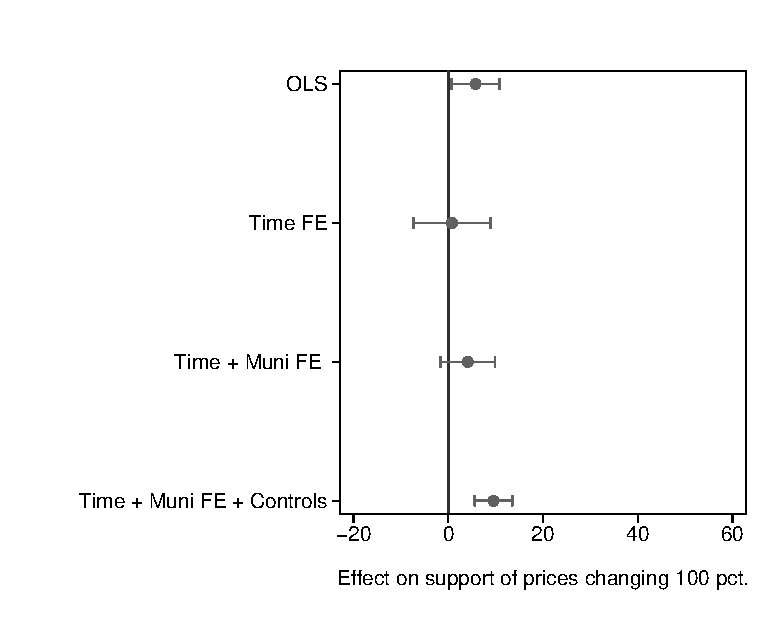
\includegraphics[width=1\textwidth]{../../figures/pooled_effects.eps} 
    \column{0.5\textwidth} \pause
		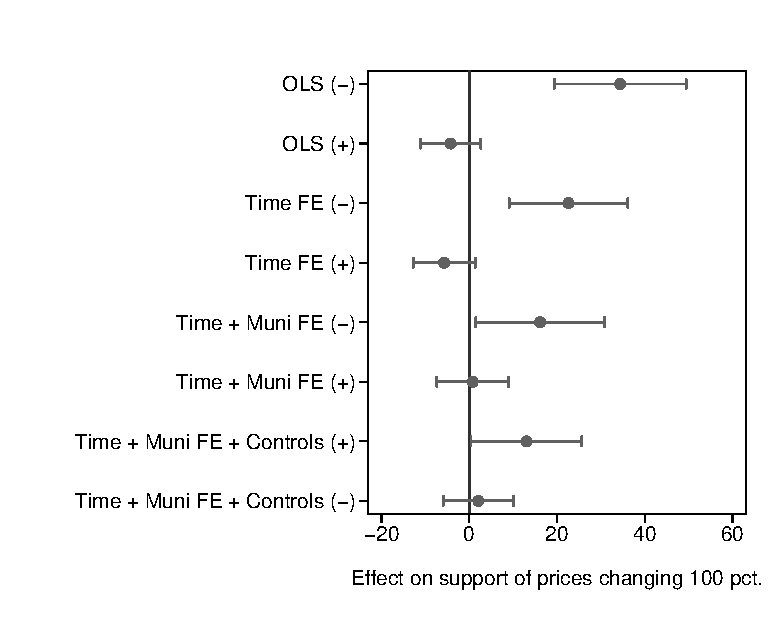
\includegraphics[width=1\textwidth]{../../figures/posneg_effects.eps}
		\end{columns} 		\pause
		
	\centering{	\footnotesize{Controls: Unemployment, tax-level, violent crime, theft.}} 
\end{frame}	

\begin{frame}
%{Population based results}
	\begin{center}
			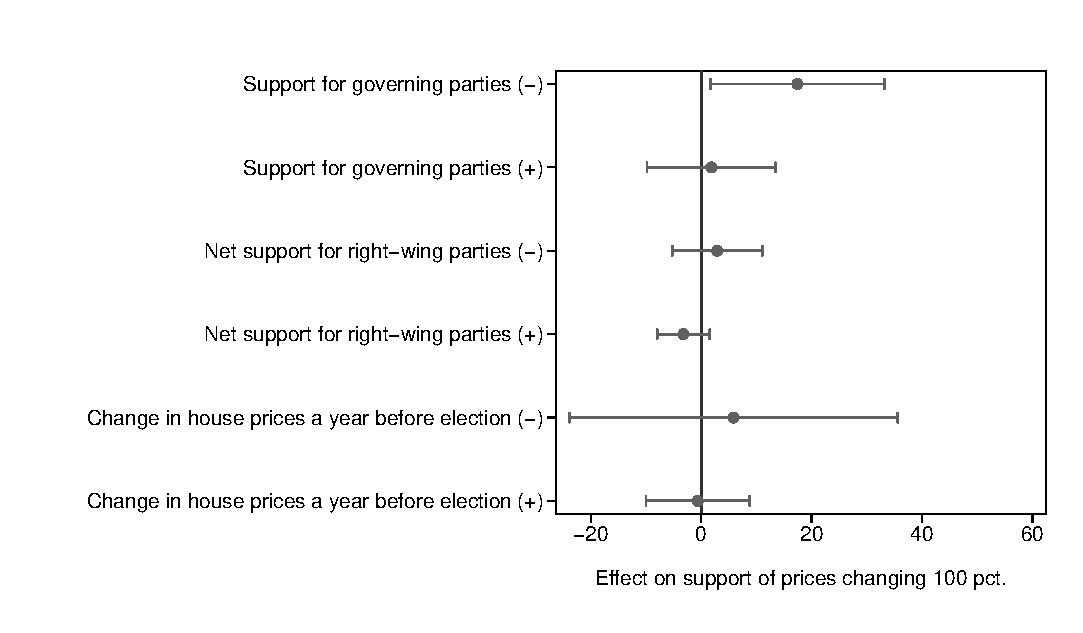
\includegraphics[width=0.6\textwidth]{../../figures/robust.eps}
	\end{center}
\end{frame}	

\begin{frame}
%{Survey based results}
	\begin{columns}
	\column{0.5\textwidth}
		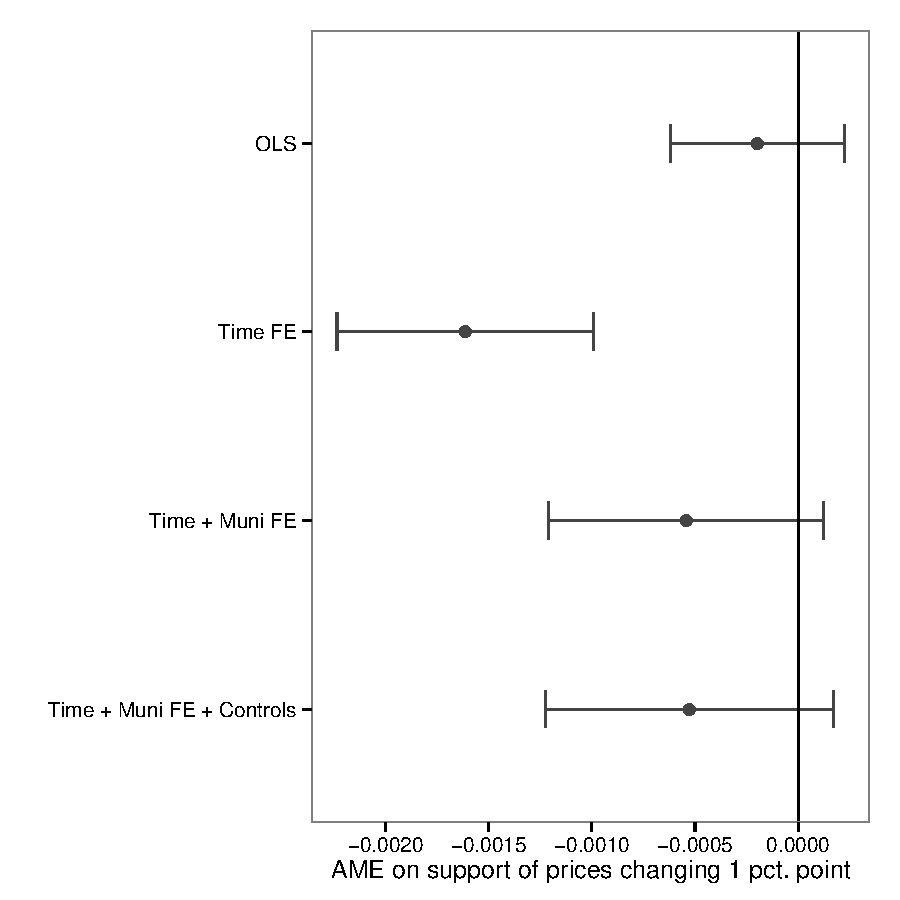
\includegraphics[width=1\textwidth]{../../figures/surveys_effplot1} 
    \column{0.5\textwidth} \pause
		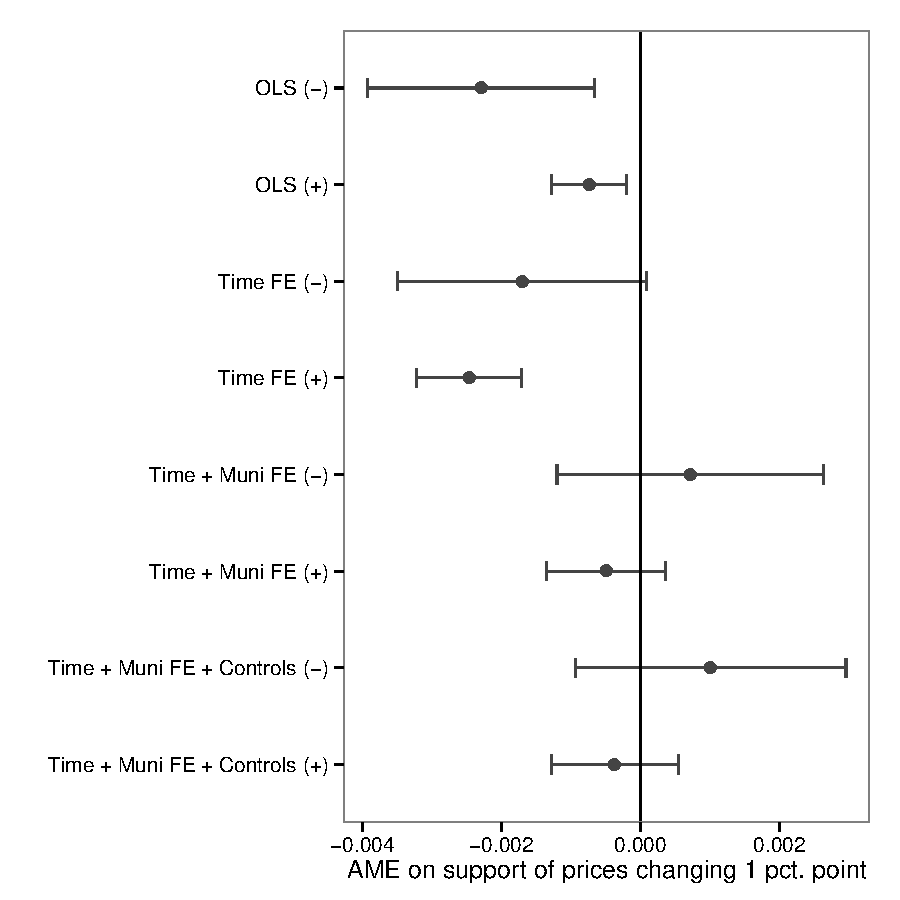
\includegraphics[width=1\textwidth]{../../figures/surveys_effplot2}
		\end{columns} 		
 \end{frame}	

\section{Discussion}

	\begin{frame}
	%{What is going on?}
	We have shown evidence suggesting that falling - but not rising - house prices hurt incumbents in Denmark.
	
	\vspace{0.2in} \pause
	
	\begin{itemize}
		\item is this convincing?
		\item what other analyses would you like to see?
		\item which interesting (theoretical and real world) implications do you think this has?
		\item do you think this is a case where personal economic grievances matter? 
	\end{itemize}	
		
	\end{frame}		

\begin{frame}
	\bibliography{litliste}
		\bibliographystyle{apsr}
\end{frame}


\end{document}